% Created 2016-12-07 mié 14:29
% Intended LaTeX compiler: pdflatex
\documentclass[11pt]{article}
\usepackage[utf8]{inputenc}
\usepackage[T1]{fontenc}
\usepackage{graphicx}
\usepackage{grffile}
\usepackage{longtable}
\usepackage{wrapfig}
\usepackage{rotating}
\usepackage[normalem]{ulem}
\usepackage{amsmath}
\usepackage{textcomp}
\usepackage{amssymb}
\usepackage{capt-of}
\usepackage{hyperref}
\author{Marc Corrales Berjano}
\date{\today}
\title{Using Emacs Orgmode as a Lab Notebook}
\hypersetup{
 pdfauthor={Marc Corrales Berjano},
 pdftitle={Using Emacs Orgmode as a Lab Notebook},
 pdfkeywords={},
 pdfsubject={},
 pdfcreator={Emacs 24.3.1 (Org mode 9.0.1)}, 
 pdflang={English}}
\begin{document}

\maketitle
\tableofcontents

\begin{itemize}
\item There is an somewhat functional version for VIM
\item There is emulation of vim in EMACS (eVIl-mode) people seem quite happy with it.
\end{itemize}

\section{Example 1 A typical day at the bench.}
\label{sec:orga70ef69}
Purpose :: The experiment that we are going to do is to know if the geeky gene (GG1)
is \textbf{overexpressed} in the memebers of this lab.

\subsection{{\bfseries\sffamily DONE} Order Oligos}
\label{sec:org446e428}
\begin{itemize}
\item I ordered the oligos for the geeky gene 1 (GG1)
\begin{itemize}
\item Fwd: GATGGGTACTGGTACAGT
\item Rev: TTTACGAGTCGTACGGA
\end{itemize}
\end{itemize}

\subsection{{\bfseries\sffamily TODO} Obtain piece of tissue of the members of the lab}
\label{sec:org463a915}
\begin{itemize}
\item I use scisors and formol as explained in \href{PNAS-1962-Gross-1014-22.pdf}{This new article}
\item The desired culture of the tissues should look like: (C-u C-c C-x C-v)
\end{itemize}

\begin{center}
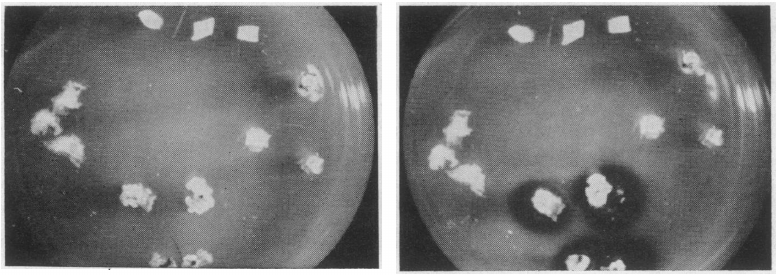
\includegraphics[width=.9\linewidth]{disgusting.png}
\end{center}

\begin{center}
\begin{tabular}{lr}
Member & weigth (g)\\
\hline
HC & 2.1\\
AR & 2.8\\
RC & 3.2\\
EV & 3.4\\
PC & 4.2\\
MC & 3.8\\
CR & 2.8\\
AT & 3.2\\
ET & 3.5\\
\end{tabular}
\end{center}



\begin{itemize}
\item Guillaume wanna participate or be the postive control?
\item Good education: Put yourself last Marc!
\end{itemize}
\subsection{{\bfseries\sffamily DONE} Obtain negative controls}
\label{sec:org2e71efc}
\begin{itemize}
\item I obtain tissue from the people that are araund the lab. Simple random
\end{itemize}
sample with a little convenience bias. 

\begin{center}
\begin{tabular}{lr}
People & Weigth (g)\\
\hline
TianTian & 2.5\\
Marc LC & 3.1\\
Alexandra & 2.8\\
\hline
\end{tabular}
\end{center}

The negative controls are the FIRST step!!! 
\subsection{{\bfseries\sffamily TODO} Facs non fatty cells}
\label{sec:org6c40db2}
\begin{itemize}
\item Disgregate the tissue with collagenase 37C 15 min.
\item Incubate cells with antibody Fairy (rcognices the receptor of Adipocites). 1h
\end{itemize}
in agitation.
\begin{itemize}
\item Bring to the facility
\end{itemize}

\subsection{{\bfseries\sffamily TODO} Extract DNA}
\label{sec:org362900c}
\begin{itemize}
\item I extract the DNA from each sample from FACS with Qiagen Blood and tissue Kit
\end{itemize}
following their recomendations. ref? 
\begin{itemize}
\item I resuspend in 40 ul EB
\end{itemize}

\begin{center}
\begin{tabular}{lrl}
Member & conc (ng/ul) & Total\\
\hline
HC & 20.1 & \\
AR & 20.8 & \\
RC & 30.2 & \\
EV & 30.4 & \\
PC & 40.2 & \\
MC & 30.8 & \\
CR & 20.8 & \\
AT & 30.2 & \\
ET & 30.5 & \\
\hline
\end{tabular}
\end{center}

\begin{itemize}
\item Total DNA ?
\end{itemize}
\subsection{{\bfseries\sffamily TODO} PCR}
\label{sec:orgb6158ba}
\begin{itemize}
\item Print it to carry to the bench.
\end{itemize}

\begin{center}
\begin{tabular}{lrl}
Component & Amount per 100 ul & 100 PCRs\\
\hline
Bfr 5X & 20 & 2 mL\\
dNTPs & 2 & 200 ul\\
Primers & 50 & -\\
gDNA & 4 ul & 400 ul\\
Phusion & 1 ul & 100 ul\\
H20 & 23 & 2.2 mL\\
\hline
 & Total  100 ul & \\
\end{tabular}
\end{center}

\subsection{{\bfseries\sffamily TODO} Run Gel}
\label{sec:org95ba535}
\begin{itemize}
\item The Gel shows that the gene has amplified 7 people. I made the
\end{itemize}
quantification with geekQuant.(Of course I havent used a loading control,
because I am a cowboy).

\begin{center}
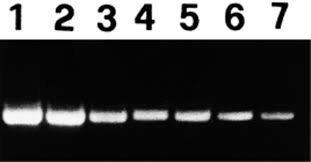
\includegraphics[width=.9\linewidth]{gel.jpg}
\end{center}

\begin{center}
\label{tab:org4c52783}
\begin{tabular}{rlr}
Num & Name & rel\(_{\text{exp}}\)\\
\hline
1 & Guillaume & 4.1\\
2 & Arantxa & 3.8\\
3 & Eduard & 3.4\\
4 & Pol & 3.0\\
5 & Albert & 3.0\\
6 & HC & 2.8\\
7 & Tiantian & 0.0\\
\end{tabular}
\end{center}

\subsection{{\bfseries\sffamily TODO} Make Figure}
\label{sec:org7053296}

\begin{itemize}
\item Lets make a barplot with the results
\end{itemize}
\begin{verbatim}
barplot(geek$rel_exp,names.arg=geek$Name,las=3, col=rainbow(20))
\end{verbatim}

\begin{center}
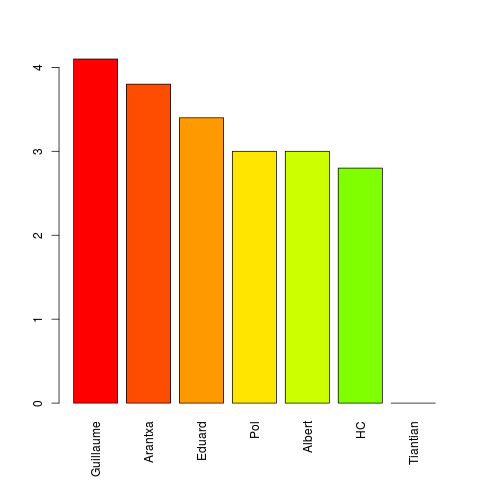
\includegraphics[width=.9\linewidth]{geektbl.png}
\end{center}

\subsection{{\bfseries\sffamily TODO} Save a pdf copy}
\label{sec:org4090ad4}
Backups are important!!!
\href{orgnotebook.pdf}{Link to the pdf}
\section{Example 2 A typical day at the computer}
\label{sec:orgb9d827e}
\begin{itemize}
\item I will make an exaple for someone doing data analysis since I dont know which
\end{itemize}
are the advantages to 'real developping'.
\subsection{{\bfseries\sffamily TODO} Start to track the project in git}
\label{sec:org643b774}
\subsection{{\bfseries\sffamily TODO} Get the data}
\label{sec:orgd866f2f}
\subsection{{\bfseries\sffamily TODO} Clean and prepare the Data}
\label{sec:orgfe258e0}
\subsection{{\bfseries\sffamily TODO} Explore the Data, Plot , statistics}
\label{sec:org672771a}
\subsection{{\bfseries\sffamily TODO} Send a report, publish, export}
\label{sec:org1de3792}
\section{Example 3 A typical day writing a paper}
\label{sec:org8f0c8fc}
\end{document}
